\documentclass[11pt,a4paper,titlepage,oneside]{report}
\input{../Toolbox/toolbox.tex}

\setcounter{tocdepth}{3}
\graphicspath{{../Images/}}

\newcommand{\tuileActive}{tuile active \includegraphics[scale=0.15]{icones/icones_jetonTuileActive} }
\newcommand{\tuilesActives}{tuiles actives \includegraphics[scale=0.15]{icones/icones_jetonTuileActive} }

\newcommand{\tuileBloquee}{tuile bloquée \includegraphics[scale=0.15]{icones/icones_jetonTuileBloquee} }
\newcommand{\tuilesBloquees}{tuiles bloquées \includegraphics[scale=0.15]{icones/icones_jetonTuileBloquee} }
\newcommand{\compteurManche}{\textcolor{OliveGreen}{compteur de manche }}

\newcommand{\faceValeur}{face valeur \includegraphics[scale=0.5]{obstacles/faceValeur/faceValeurs_bleu_1}}
\newcommand{\faceObstacle}{face obstacle \includegraphics[scale=0.5]{obstacles/faceObstacle/faceObstacles_bleu_rocher}}

\newcommand{\marqueurObstacle}{marqueur d'obstacle \includegraphics[scale=0.2]{icones/fond_obstacles}}
\newcommand{\marqueursObstacles}{marqueurs d'obstacle \includegraphics[scale=0.2]{icones/fond_obstacles}}

\newcommand{\jetonObstacle}{jeton obstacle \includegraphics[scale=0.3]{regle/obstacles}}
\newcommand{\jetonsObstacles}{jetons obstacles \includegraphics[scale=0.3]{regle/obstacles}}

\newcommand{\jetonMeteo}{jeton meteo 
\includegraphics[scale=0.2]{jetonsMeteo/verso}}
\newcommand{\jetonsMeteo}{jetons meteo 
\includegraphics[scale=0.2]{jetonsMeteo/verso}}

\newcommand{\eau}{\includegraphics[scale=0.02]{jetonsJoueurs/eau} }
\newcommand{\foudre}{\includegraphics[scale=0.02]{jetonsJoueurs/foudre} }
\newcommand{\nature}{\includegraphics[scale=0.02]{jetonsJoueurs/nature} }
\newcommand{\terre}{\includegraphics[scale=0.02]{jetonsJoueurs/terre} }
\newcommand{\vent}{\includegraphics[scale=0.02]{jetonsJoueurs/vent} }

\newcommand{\arbre}{\includegraphics[scale=0.15]{icones/icones_arbre} }
\newcommand{\rocher}{\includegraphics[scale=0.15]{icones/icones_rocher} }
\newcommand{\tronc}{\includegraphics[scale=0.15]{icones/icones_tronc} }

\pagestyle{plain}

\title{\includegraphics[scale=2]{titre/titre}}
\edr
\begin{document}
	\dateVersion{v1.0.0}
	\maketitle
	\tableofcontents
	\pagebreak
	
	\input{intro}
	\section*{Matériel} \label{sec:Matériel}
\addcontentsline{toc}{section}{Matériel}

Ce jeu est composé de:
\begin{itemize}
\item 18x \jetonsObstacles, recto verso, répartis en 6 couleurs ( \includegraphics[scale=0.15]{obstacles/fond_bleu}, 
\includegraphics[scale=0.15]{obstacles/fond_gris}, \includegraphics[scale=0.15]{obstacles/fond_rouge}, \includegraphics[scale=0.15]{obstacles/fond_jaune}, \includegraphics[scale=0.15]{obstacles/fond_vert}, \includegraphics[scale=0.15]{obstacles/fond_violet} ). D'un côté des valeurs, de l'autre des obstacles. Les valeurs rapportent des points directement, les obstacles en fin de partie.
\item 3x \marqueursObstacles, avec les différents obstacles que vous pouvez rencontrer (\arbre, \tronc, \rocher)
\item 15x \jetonsMeteo, qui permettent de mesurer le temps qui passe.
\item 6x randonneurs, avec des couleur différentes (\includegraphics[scale=0.08]{meeples/meepleBleu}, \includegraphics[scale=0.08]{meeples/meepleGRis}, \includegraphics[scale=0.08]{meeples/meepleRouge}, \includegraphics[scale=0.08]{meeples/meepleJaune}, \includegraphics[scale=0.08]{meeples/meepleVert}, \includegraphics[scale=0.08]{meeples/meepleViolet})
\item 66x cartes recto-verso. Les cartes sont construites ainsi:
\begin{itemize}
\item[*] le verso \includegraphics[scale=0.25]{regle/carteVerso} comporte un randonneur de couleur. Il permet d'indiquer le randonneur qui va se déplacer
\item[*] le recto \includegraphics[scale=0.25]{regle/carteRecto} comporte deux informations: au centre, l'effet immédiat et dans les coins les informations de points en fin de partie.
\end{itemize}
\item un plateau central, divisé en plusieurs zones.
\end{itemize}

De plus, chaque joueur possède:
\begin{itemize}
\item un plateau pour indiquer les multiplicateurs d'actions.
\item 9 jetons de son esprit
\item 6 tuiles recto-verso \includegraphics[scale=0.25]{regle/tuiles}, une pour chaque action possible. D'un côte, l'action est accessible (\tuileActive), de l'autre l'action est bloquée (\tuileBloquee).
\end{itemize}
\FloatBarrier

	\section*{But du jeu}
\label{butDuJeu}
\addcontentsline{toc}{section}{But du jeu}
	
	\section*{Mise en place}
\addcontentsline{toc}{section}{Mise en place}

\subsection*{Premier joueur}
\addcontentsline{toc}{subsection}{Premier joueur}
	
	\section*{Le déroulement de la partie} \label{sec:tourDeJeu}
\addcontentsline{toc}{section}{Le déroulement de la partie}
La partie se déroule en 15 manches, durant lesquelles chaque joueur va jouer un tour.

\subsection*{Le tour d'un joueur} \label{sec:tourDeJoueur}
\addcontentsline{toc}{subsection}{Le tour d'un joueur}
Le tour de jeu se divise en 3 phases successives, où le joueur :
\subsubsection*{\includegraphics[scale=1]{icones/phase1} \\ Peut retourner deux tuiles}
Durant cette phase \textbf{facultative}, le joueur peut retourner deux \tuilesActives sur leur face \textit{bloquée}. Dans ce cas, il retourne une \tuileBloquee sur sa face \textit{active}.

\subsubsection*{\includegraphics[scale=1]{icones/phase2} \\ Doit jouer une tuile}
Durant cette phase \textbf{obligatoire},
\begin{enumerate}
\item le joueur choisit une \tuileActive et la retourne sur sa face \textit{bloquée},
\item puis il joue l'action correspondante, en appliquant le multiplicateur associé.
\item Tous les joueurs retournent cette tuile et une autre
\end{enumerate}

\acompleter{EXEMPLE}
\subsubsection*{\includegraphics[scale=1]{icones/phase3} \\ Peut jouer une carte}
Durant cette phase \textbf{facultative}, le joueur peut jouer une carte de sa main. Selon l'icône au centre de la carte, le joueur va:
\begin{enumerate}
\item \includegraphics[scale=0.25]{icones/action} jouer une action supplémentaire
\item \includegraphics[scale=0.25]{icones/fond_obstacles} gagner un obstacle
\item \includegraphics[scale=0.25]{icones/icones_5} marquez des points
\end{enumerate}

Une fois que le joueur a joué son tour, c'est au tour du joueur à sa gauche. Une fois que tous les joueurs ont joué leur tour, passer à l'étape de fin de manche.

\subsection*{La fin de la manche} \label{sec:finDeManche}
\addcontentsline{toc}{subsection}{La fin de la manche}
Pour marquer la fin de la manche, déplacer le \compteurManche d'une case et appliquer l'effet:
\begin{itemize}
\item \includegraphics[scale=0.8]{jetonsMeteo/jetonEclair}: retournez toutes vos tuiles sur la face \textit{active}, sauf une sur sa face \textit{bloquee}
\item \includegraphics[scale=0.8]{jetonsMeteo/jetonTonnerre}: écartez définitivement une de vos tuiles
\item \includegraphics[scale=0.8]{jetonsMeteo/jetonSoleil}: profitez d'un tour de répit, rien ne se passe
\item \includegraphics[scale=0.8]{jetonsMeteo/jetonVent}: choisissez entre donner une carte à votre voisin de gauche ou perdre \textbf{3 points}
\item \includegraphics[scale=0.8]{jetonsMeteo/jetonPluie}: choisissez entre diminuer de 1 un des multiplicateur ou perdre \textbf{3 points}
\end{itemize}

\subsection*{Détail des actions} \label{sec:actions}
\addcontentsline{toc}{subsection}{Détail des actions}
Toutes les actions, à l'exception du joker, suivent le même fonctionnement: l'effet est appliqué autant de fois que le valeur du multiplicateur associé.
\subsubsection*{\includegraphics[scale=0.3]{icones/icones_deplacerMeeples} \\ Déplacer des randonneurs}
\important{\begin{itemize}
\item[*]La couleur du randonneur est donnée par la carte au sommet de la pioche.
\item[*]Si les couleurs de l'obstacle et du randonneur sont les même, doublez la récompense.
\item[*] Maximum 3 déplacements par action.
\end{itemize}}

Cette action va permettre de faire rebondir des randonneurs pour marquer des points. La couleur du randonneur qui se déplace est donnée par la carte au sommet de la pioche. Si les couleurs de l'obstacle et du randonneur sont les même, doublez la récompense. Pour déplacer un randonneur:
\begin{enumerate}
\item Déplacez le randonneur qui a la même couleur que le sommet de la pioche, en suivant le chemin, dans la direction de votre choix, jusqu'à rencontrer un obstacle
\item selon la nature de l'obstacle:
\begin{itemize}
\item[*] Si l'obstacle est un autre randonneur, le premier s'arrête et le deuxième part en suivant le chemin,
\item[*] Si l'obstacle est le bord du terrain, le randonneur rebondit et repart dans une autre direction
\item[*] Si l'obstacle est une \faceValeur, marquez les points correspondants, retournez l'obstacle et faite repartir le randonneur dans une autre direction.
\item[*] Si l'obstacle est une \faceObstacle, augmentez le jeton sur l'echelle de l'obstacle correspondante, retournez l'obstacle et faite repartir le randonneur dans une autre direction.
\end{itemize}
\item Défaussez la carte du dessus de la pioche.
\end{enumerate}

\acompleter{EXEMPLE}

\subsubsection*{\includegraphics[scale=0.3]{icones/icones_piocherCarte} \\ Piocher des cartes}
\important{La taille de la main est limitée à 3 cartes.}
Piochez autant de cartes que la valeur de votre multiplicateur. Défaussez pour n'avoir que trois cartes en mains.

\subsubsection*{\includegraphics[scale=0.3]{icones/icones_multiplicateurNegatif} \\ Diminuer des multiplicateurs}
Diminuez de 1 un multiplicateur d'un autre joueur. Si vous acez plusieurs actions, vous pouvez répartir vos actions comme vous voulez (le même joueur, la même piste, des joueurs différents, des pistes différentes).

\subsubsection*{\includegraphics[scale=0.3]{icones/icones_multiplicateurPositif} \\ Augmenter des multiplicateurs}
Augmentez un de vos multiplicateurs. Si vous avez plusieurs actions, vous pouvez les répartir comme vous voulez.

\subsubsection*{\includegraphics[scale=0.3]{icones/icones_obstacle} \\ Modifier l'ordre des obstacle}
Échangez de place deux \marqueursObstacles.

\subsubsection*{\includegraphics[scale=0.3]{icones/icones_joker} \\ Remplacer une action}
\important{Ignorez les multiplicateurs.}
Effectuez n'importe quelle action, une seule fois.	
	\section*{Fin de partie}
\addcontentsline{toc}{section}{Fin de partie}

\subsection*{Comptage des points}
\addcontentsline{toc}{subsection}{Comptage des points}

	\section*{Décompte final} \label{sec:comptagePoints}
\addcontentsline{toc}{section}{Décompte final}


\end{document}
